\chapter{はじめに}
\section{まえがき}
はじめまして、エンジニアを目指している鹿さんと申します.\\
今回初めて本を出すことになりまして、GolangによりICMPとARPを用いたネットワーク内のデバイス数を取得する方法を書いてみました.
ICMPとはpingコマンドなどに使われるプロトコルのことで、ARPとはネットワーク上のMACアドレスを取得するするためのプロトコルです.
この本ではそれぞれ簡単な説明の後、pingやarpscanのようなLinuxコマンドを用いずに実装していきます.\\
本を執筆することも、ネットワーク系技術についても不慣れなため、不自然さや間違い等あるかもしれませんが、是非とも生暖かい目で応援よろしくお願いします.

\chapter{ICMP・ARPの解説}
ここではICMP・ARPそれぞれについての解説と、この2つのプロトコルの違いについて解説していきます。
\section{ICMPについて}
ICMPの概要、パケット構成、タイプについて解説していきます
\subsection{概要}
Internet Control Message Protocol(ICMP)は、ネットワーク通信の問題を診断するためにネットワークデバイスが使用するネットワーク層のプロトコルです\cite{icmp}。 \\
ICMPには、問い合わせ用のQueryとエラー発生時に発行されるErrorの2種類のメッセージが存在しており、
主にデータが目的の宛先にタイムリーに到達しているかどうかを判断するために使用されています。
ICMPが使われている代表的なLinuxコマンドにpingがあります。
\begin{figure}[H]
    \centering
    
\includegraphics[width=10cm]{image/02-Body/icmp_image.jpeg}
    \caption{ICMPのイメージ}
    \label{icmp_image}
\end{figure}
\subsection{パケット構成}
パケット構成は次の図のようになっています。\\
\begin{shaded}
    \begin{verbatim}
    0                   1                   2                   3
    0 1 2 3 4 5 6 7 8 9 0 1 2 3 4 5 6 7 8 9 0 1 2 3 4 5 6 7 8 9 0 1
    +-+-+-+-+-+-+-+-+-+-+-+-+-+-+-+-+-+-+-+-+-+-+-+-+-+-+-+-+-+-+-+-+5
    |     Type      |     Code      |          Checksum             |
    +-+-+-+-+-+-+-+-+-+-+-+-+-+-+-+-+-+-+-+-+-+-+-+-+-+-+-+-+-+-+-+-+
    |     Data ...
    +-+-+-+-+-
  \end{verbatim}
\end{shaded}
構成内のそれぞれの要素は次の表のようになっています。
\begin{table}[bth]
    \begin{center}
    \caption{ICMPパケットの要素}
        \label{icmp-table}
            \begin{tabular}{|c|c|c|c|} \hline
                フィールド & ビット数 & 内容 \\ \hline
                Type & 8bit & 機能(タイプ)の番号 \\ \hline
                Code & 8bit & Typeの詳細な機能コード(オプションのようなもの) \\ \hline
                Checksum & 16bit & エラーの有無を確認 \\ \hline
                Data & 可変長 & Typeごとに必要なデータが加わる\\ \hline
            \end{tabular}
    \end{center}
\end{table}
特にpingコマンドで使われるEcho Typeでは、DateにReplyとの対応付けとして使用できる識別子・番号であるIdentifier、Sequence Numberがそれぞれ16bitずつ割り当てられます。

\subsection{Typeについて}
Typeは全部で13個存在し、それぞれが別の機能を持っています。
pingコマンドでは0と8が使われています。
\begin{table}[bth]
    \begin{center}
        \caption{ICMPのType一覧}
        \label{icmp-type}
            \begin{tabular}{|c|c|c|c|} \hline
                Type番号 & 機能\\ \hline
                0 & エコー応答 \\ \hline
                3 & 宛先不達 \\ \hline
                5 & リダイレクト要求 \\ \hline
                8 & エコー要求 \\ \hline
                11 & 時間超過 \\ \hline
                13 & タイムスタンプ要求 \\ \hline
                14 & タイムスタンプ応答 \\ \hline
                15 & 情報要求 \\ \hline
                16 & 情報応答 \\ \hline
                17 & アドレス・マスク要求 \\ \hline
                18 & アドレス・マスク応答 \\ \hline
            \end{tabular}
    \end{center}
\end{table}

\section{ARPについて}
\subsection{概要}
Address Resolution Protocol(ARP)とは、IPアドレスからMACアドレスを求めるために利用されるデータリンク層で動作するプロトコルのことです。\\
要求と応答である「ARPリクエスト」と「ARPレスポンス」の2種類のメッセージが存在し、主にイーサネット上での物理的な通信の際に対象のMACアドレスとIPアドレスの対応表を作成するのに使われます。
なぜIPアドレスがあるにもかかわらずMACアドレスが必要なのかと言いうと、IPアドレスが必要となるのはネットワーク層での話であり、データリンク層ではMACアドレスを元にターゲットを特定するためです。
ARPが使われている代表的なLinuxコマンドとして、LAN内のIPアドレスとMACアドレスの一覧を表示するarpscanがあります。


\subsection{パケット構造}
ARPパケットはEthernet形式のフレームでイーサネットヘッダによってカプセル化されています。
また、イーサネットヘッダのタイプコード0x0806でデータ部分がARPメッセージであることを表します\cite{arp_format}\cite{yokuwakaru}。
\begin{figure}[H]
    \centering
    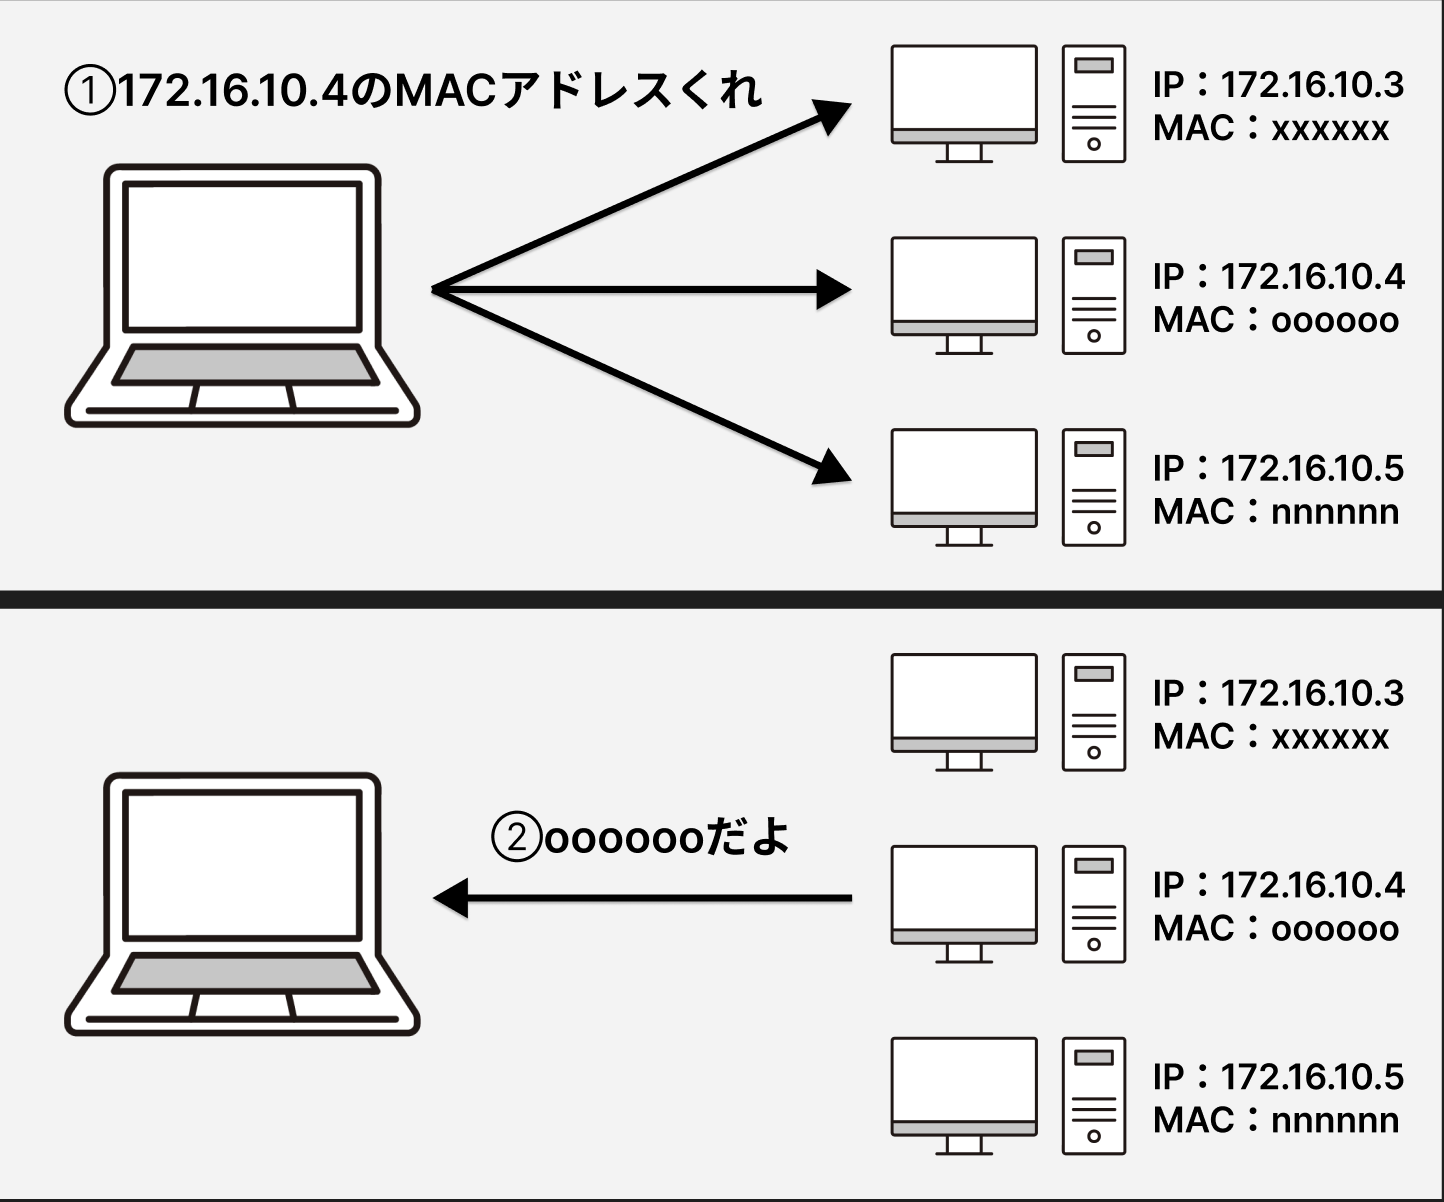
\includegraphics[width=7cm]{image/02-Body/arp_image.png}
    \caption{ARPのイメージ}
    \label{arp_image}
\end{figure} 
% \begin{figure}[H]
%     \centering
%     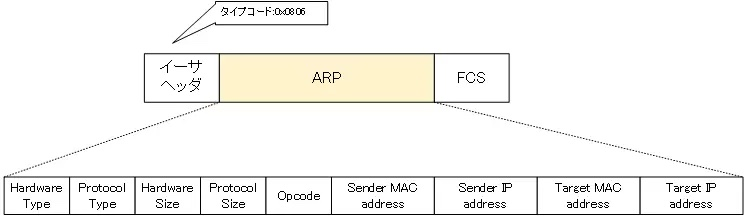
\includegraphics[width=10cm]{image/02-Body/arp_format01.jpeg}
%     \caption{ARPフォーマット\cite{arp_format}}
%     \label{arp_format}
% \end{figure}
\begin{shaded}
    \begin{verbatim}
    0                   1                   2                   3
    0 1 2 3 4 5 6 7 8 9 0 1 2 3 4 5 6 7 8 9 0 1 2 3 4 5 6 7 8 9 0 1
    +-+-+-+-+-+-+-+-+-+-+-+-+-+-+-+-+-+-+-+-+-+-+-+-+-+-+-+-+-+-+-+-
    |          Hardware Type      |          Protocol Type         |
    +-+-+-+-+-+-+-+-+-+-+-+-+-+-+-+-+-+-+-+-+-+-+-+-+-+-+-+-+-+-+-+-
    | Hardware Size| Protocol Size|            Opcode              |
    +-+-+-+-+-+-+-+-+-+-+-+-+-+-+-+-+-+-+-+-+-+-+-+-+-+-+-+-+-+-+-+-
    |                      Sendr MAC address                       |
    +-+-+-+-+-+-+-+-+-+-+-+-+-+-+-+-+-+-+-+-+-+-+-+-+-+-+-+-+-+-+-+-
    |    Sendr MAC address(続き)   |       Sendr IP address         |
    +-+-+-+-+-+-+-+-+-+-+-+-+-+-+-+-+-+-+-+-+-+-+-+-+-+-+-+-+-+-+-+-
    |    Sender IP address(続き)   |       Target MAC address       |
    +-+-+-+-+-+-+-+-+-+-+-+-+-+-+-+-+-+-+-+-+-+-+-+-+-+-+-+-+-+-+-+-
    |                    Target MAC address(続き)                   |
    +-+-+-+-+-+-+-+-+-+-+-+-+-+-+-+-+-+-+-+-+-+-+-+-+-+-+-+-+-+-+-+-
    |                      Target IP address                       |
    +-+-+-+-+-+-+-+-+-+-+-+-+-+-+-+-+-+-+-+-+-+-+-+-+-+-+-+-+-+-+-+-
  \end{verbatim}
\end{shaded}
それぞれのフィールドのビット数、内容は次のようになっています。
Ethernet、IPv4の環境下では、Hardware Type、Protocol Type、Hardware Size、Protocol Sizeは固定値となります。

\begin{table}[bth]
    \begin{center}
        \caption{ARPパケットの要素\cite{arp_format}}
        \label{arp_field}
            \begin{tabular}{|c|c|c|c|} \hline
                フィールド & ビット数 & 内容\\ \hline
                Hardware Type & 16bit & イーサネットの場合、0x0001で固定\\ \hline
                Protocol Type & 16bit & IPv4の場合、0x0800で固定\\ \hline
                Hardware Size & 8bit &
                \begin{tabular}{c}
                    MACアドレスのサイズ(Byte)\\MACアドレスは48bit=6Byteなので、0x06
                \end{tabular}\\ \hline
                Protocol Size & 8bit & 
                \begin{tabular}{c}
                    IPアドレスのサイズ(Byte)\\ IPアドレス(IPv4)は32bit=4Byteなので、0x04
                \end{tabular}\\ \hline
                Opcode & 16bit &
                \begin{tabular}{c}
                    ARPリクエスト:0x0001\\ ARPレスポンス:0x0002
                \end{tabular}\\ \hline
                Sender MAC address & 48bit & 送信元MACアドレス\\ \hline
                Sender IP address & 32bit & 送信元IPアドレス\\ \hline
                Target MAC address & 48bit & ターゲットMACアドレス\\ \hline
                Target IP address & 32bit & ターゲットIPアドレス\\ \hline
            \end{tabular}
    \end{center}
\end{table}

% \section{それぞれの比較}
% 次の表のようにまとめると、比較するのもおこがましいくらい違いますね。
% なんで比較したんでしょう、って感じになりますがこれらをうまく使うとネットワーク内のデバイス数を取得できるようになります。
% ということでようやく本題、「ICMP、ARPを使ってネットワーク内のデバイスを取得する」をやっていきます。

% \begin{table}[bth]
%     \begin{center}
%         \caption{ICMPとARPの比較}
%         \label{chapteromparison-table}
%             \begin{tabular}{|c|c|c|} \hline
%                  & ICMP & ARP \\ \hline
%                 OSI参照モデル & ネットワーク層 & データリンク層 \\ \hline
%                 目的 & ネットワークの診断 & MACアドレスの取得 \\ \hline
%                 対象 & ネットワーク機器 & LAN内全体 \\ \hline
%                 ルータ & 越える & 越えない \\ \hline
%             \end{tabular}
%     \end{center}
% \end{table}

\chapter{ICMP、ARPを使ってネットワーク内のデバイスを取得する with Golang}
\section{ARPバージョン}
まずはARPの方から実装していこうと思います。\\
やることとしては、Linuxコマンドであるarpscanを実装する手順とほとんど同じです。
GoogleがGitHubで公開しているサンプルプログラムを参考にしました\cite{arpscan}。
ARPはルータを越えることができないので、同一ネットワーク内が前提です。また、今回はmoduleの設定等については省略します。
今回実装する処理の流れは以下のようになります。
\begin{enumerate}
    \item ホストのネットワークインターフェイスを全て取得
    \item 1で取得した中からIPv4を使用しているインターフェイスを検索
    \item 2で使用しているアドレスからそのネットワークで扱えるすべてのIPを取得
    \item ネットワークのすべてのIPに対してARPリクエストを送信
    \item ARPレスポンスの数を計測
    \item 表示
\end{enumerate}
\subsection{ホストのネットワークインターフェイスを全て取得}
まずはnetパッケージのInterfaces関数によりインターフェイスのリストを取得します。
ここでエラーが発生した場合はpanicを発行して終了させます。
\begin{tcolorbox}[breakable]
    \begin{verbatim}
1 func main() {
2   // すべてのインターフェイスのリストを取得します
3	ifaces, err := net.Interfaces()
4	if err != nil {
5	    panic(err)
6	 }
7 }
    \end{verbatim}
\end{tcolorbox}

\subsection{取得したリストからIPv4を使用しているインターフェイスを検索}
IPv4のアドレスを使用しているインターフェイスを検索し、IPアドレスとサブネットマスクを取得します。
これらはインターフェイス1つずつ行われ、取得できなかった場合やlocalhostであった場合はエラーを返します。
\begin{tcolorbox}[breakable]
    \begin{verbatim}
1 // ARPリクエスト/リプライを使用して、
2 // 個々のインターフェイスをスキャンします
3 func scan(iface *net.Interface) (int, error) {
4   // IPv4アドレスを取得する
5   var addr *net.IPNet
6   if addrs, err := iface.Addrs(); err != nil {
7       return 0, err
8   } else {
9       for _, a := range addrs {
10       	if ipnet, ok := a.(*net.IPNet); ok {
11			    if ip4 := ipnet.IP.To4(); ip4 != nil {
12                  addr = &net.IPNet{
13		    		    IP:   ip4,
14	        		Mask: ipnet.Mask[len(ipnet.Mask)-4:],
15	        		}
16		        	break
17		        }
18	        }
19	    }
20  }
21  // インターフェイスのアドレスが正しいかどうかをチェックします。
22 	if addr == nil {
23  	return 0, errors.New("no good IP network found")
24  } else if addr.IP[0] == 127 {
25		return 0, errors.New("skipping localhost")
26 	} else if addr.Mask[0] != 0xff || addr.Mask[1] != 0xff {
27  	return 0, errors.New("mask means network is too large")
28  }
29      log.Printf(
30        "Using network range %v for interface %v",
31        addr,
32        iface.Name
33      )
34  }
    \end{verbatim}
\end{tcolorbox}

\subsection{使用しているアドレスとマスクからそのネットワークで扱えるすべてのIPを取得}
IPアドレスとサブネットマスクがわかれば、接続しているネットワークで割り当て可能なIPアドレスの範囲がわかります。
それらをoutというnet.IP型のスライスに格納します。
\begin{tcolorbox}[breakable]
    \begin{verbatim}
1 // ipsは、net.IPNetからすべてのIPv4アドレスを取得します
2 func ips(n *net.IPNet) (out []net.IP) {
3   num := binary.BigEndian.Uint32([]byte(n.IP))
4   mask := binary.BigEndian.Uint32([]byte(n.Mask))
5   network := num & mask
6   broadcast := network | ^mask
7   for network++; network < broadcast; network++ {
8	    var buf [4]byte
9		binary.BigEndian.PutUint32(buf[:], network)
10      out = append(out, net.IP(buf[:]))
11  }
12  return
13  }
    \end{verbatim}
\end{tcolorbox}

\subsection{ネットワークのすべてのIPに対してARPリクエストを送信}
先ほど上でARPのパケット構造について解説した通りにデータを格納し、各IPアドレスに対して1回送信します。
\begin{tcolorbox}[breakable]
    \begin{verbatim}
1 // writeARP は、ローカルネットワーク上の各アドレスに対する ARPリクエストを pcapハンドルに書き込みます
2 func writeARP(
3   handle *pcap.Handle, 
4   iface *net.Interface, 
5   addr *net.IPNet
6   ) error {
7       // できる限りすべてのレイヤーのフィールドを設定します
8       eth := layers.Ethernet{
9		    SrcMAC:       iface.HardwareAddr,
10	        DstMAC:       net.HardwareAddr{
12             0xff, 0xff, 0xff, 0xff, 0xff, 0xff
13          },
14          EthernetType: layers.EthernetTypeARP,
15      }
16      arp := layers.ARP{
17          AddrType:          layers.LinkTypeEthernet,
18	        Protocol:          layers.EthernetTypeIPv4,
19	        HwAddressSize:     6,
20	        ProtAddressSize:   4,
21	        Operation:         layers.ARPRequest,
22	        SourceHwAddress:   []byte(iface.HardwareAddr),
23	        SourceProtAddress: []byte(addr.IP),
24	        DstHwAddress:      []byte{0, 0, 0, 0, 0, 0},
25      }
26      // シリアライズのためのバッファとオプションを設定する
27      buf := gopacket.NewSerializeBuffer()
28      opts := gopacket.SerializeOptions{
29		    FixLengths:       true,
30	        ComputeChecksums: true,
31	    }
32	    // すべてのアドレスに対して1パケットを送信する
33	    for _, ip := range ips(addr) {
34		    arp.DstProtAddress = []byte(ip)
35		    gopacket.SerializeLayers(buf, opts, &eth, &arp)
36		    if err := handle.WritePacketData(buf.Bytes()); err != nil {
37			    return err
38		    }
39	    }
40	    return nil
41  }
    \end{verbatim}
\end{tcolorbox}

\subsection{ARPレスポンスの数を計測}
readARPはARPレスポンスを受け取り、受け取ったレスポンスの数をカウントする関数です。
受け取ったパケットが空であったり、自身の送信したパケットの場合はカウントしません。
この関数はチャネルによってstopを受け取るまで処理を繰り返します。
\begin{tcolorbox}[breakable]
    \begin{verbatim}
1 func readARP(
2   handle *pcap.Handle, 
3   iface *net.Interface, 
4   stop chan struct{}, 
5   c chan int
6 ) {
7   src := gopacket.NewPacketSource(
8       handle, layers.LayerTypeEthernet
9   )
10  in := src.Packets()
11  count := 0
12  for {
13      var packet gopacket.Packet
14      select {
15          case <-stop:
16              c <- count
17			    return
18	        case packet = <-in:
19			    arpLayer := packet.Layer(layers.LayerTypeARP)
20			    if arpLayer == nil {
21			        continue
22			    }
23			    arp := arpLayer.(*layers.ARP)
24			    if arp.Operation != 
25                  layers.ARPReply || bytes.Equal(
26                      []byte(iface.HardwareAddr), 
27                      arp.SourceHwAddress
28                  ) {
29		                // 自身が送信したパケットです
30		                continue
31	                }
32	            if arp.SourceProtAddress[
33                  len(arp.SourceProtAddress)-1
34              ] == 1 {
35				    continue
36			    }
37			    count++
38              log.Printf(
39                  "IP %v is at %v", 
40                  net.IP(arp.SourceProtAddress), 
41                  net.HardwareAddr(arp.SourceHwAddress)
42              )
43          }
44	    }
45 }
    \end{verbatim}
\end{tcolorbox}

\subsection{それぞれの関数を繋げて、表示}
ここまでで機能的なものは完成しました。
あとは一つのプログラムとして動作できるようにそれぞれの関数を繋いでいきます。
main関数、scan関数のすでに記述した部分については「・・・」で省略します。
\begin{tcolorbox}[breakable]
    \begin{verbatim}
1 func main() {ー
2       ・・・
3   // すべてのインタフェイスをスキャンします
4   // それぞれのスキャンは、別のGoroutineで実行されます
5   // スキャンが完了すると、チャネルに結果が送信されます
6   // ふさわしくないインターフェイスの場合は、エラーが発生します
7   c := make(chan int)
8   for _, iface := range ifaces {
9       go func(iface net.Interface, c chan int) {
10          if count, err := scan(&iface); err != nil {
11              log.Printf("interface %v: %v", iface.Name, err)
12          } else {
13              fmt.Println("success")
14              c <- count
15          }
16      }(iface, c)
17  }
18  fmt.Println(<-c)
19 }
20
21 // ARPリクエスト/リプライを使用して、個々のインターフェイスをスキャンします
22 // パケットを書き込めなかった場合はエラーを返します
23 func scan(iface *net.Interface) (int, error) {
24      ・・・
25      // パケットの読み取り/書き込み用に pcap ハンドルを開きます
26      handle, err := pcap.OpenLive(
27          iface.Name, 65536, true, pcap.BlockForever
28      )
29	    if err != nil {
30		    return 0, err
31	    }
32	    defer handle.Close()
33
34	    // パケットデータを読み込むためにGoroutineを起動する
35	    stop := make(chan struct{})
36	    c := make(chan int)
37	    go readARP(handle, iface, stop, c)
38	    defer close(c)
39	    // スキャンパケットをハンドルに書き出す
40	    writeARP(handle, iface, addr)
41	    time.Sleep(3 * time.Second)
42	    close(stop)
43	    count := <-c
44	    return count, nil
45 }
    \end{verbatim}
\end{tcolorbox}
これにて完成です!
それでは実際に動かしてみましょう。

\subsection{実行}
main.goをsudo権限で実行してください。
おそらく\ref{arp_get}のような結果になったかと思います。
出力の最後の方がこのプログラムで検知できたデバイス、一番最後の数字の出力が検知できたデバイス数となります。
\begin{figure}[H]
    \centering
    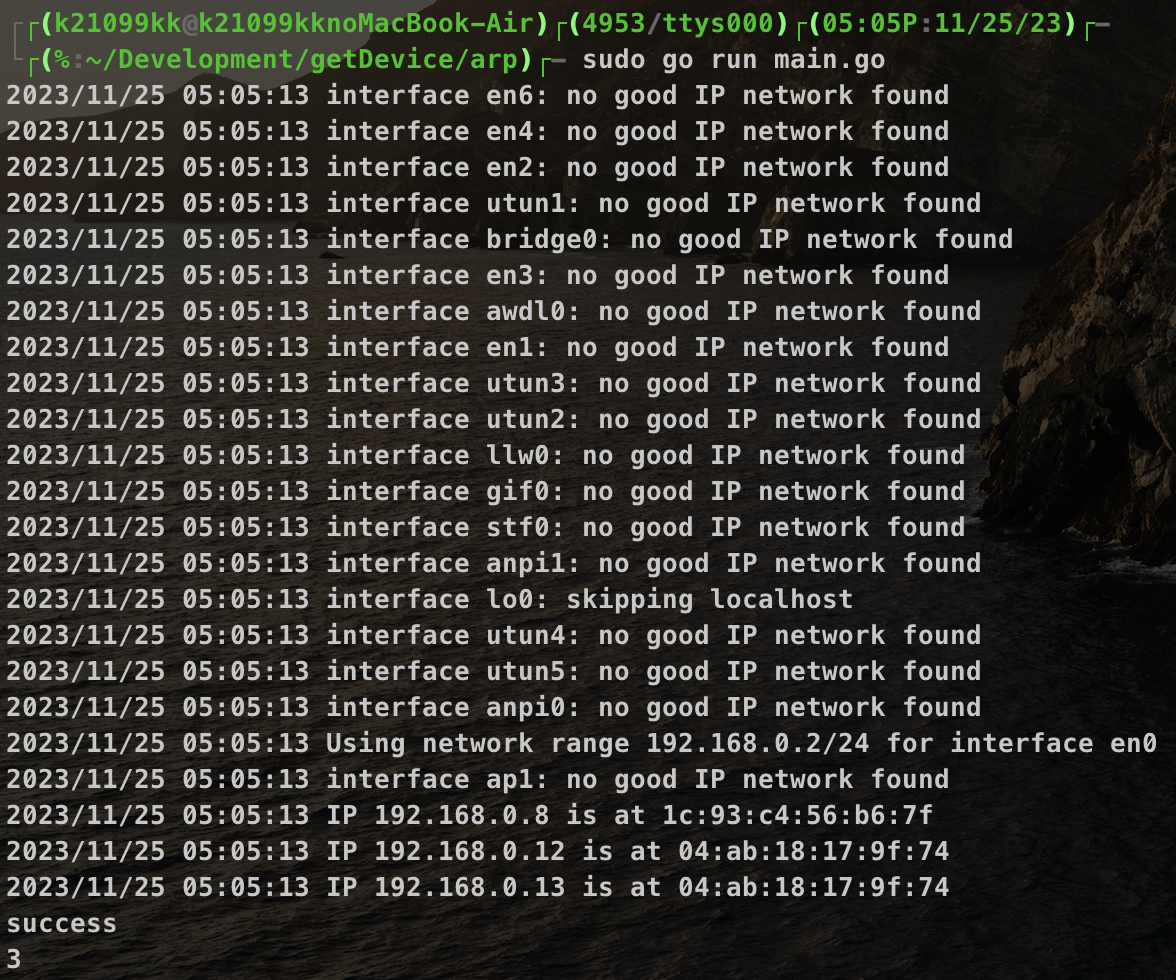
\includegraphics[width=10cm]{image/02-Body/arp_get.png}
    \caption{ICMPのイメージ}
    \label{arp_get}
\end{figure}

\section{ICMPバージョン}
次にICMPを用いて実装していきます。
こちらもARPと同じようにLinuxコマンドであるpingを実装する過程で改良していきます。
ただし、ICMPはルータを超えることができる特性を活用し、\ref{network}のような、同一LAN内で別ネットワークになっている部分に対し、ネットワークごとに接続端末数を取得していきます。
元のプログラムはpgDora56様を参考にさせていただきました\cite{pgDora56}。
実装する処理の流れは以下の通りです。
\begin{enumerate}
    \item csvファイルからネットワーク一覧を取得
    \item それぞれのネットワークで扱えるすべてのIPを取得
    \item ネットワークのすべてのIPに対してエコーTypeでICMPプロトコルを実行
    \item エコー応答の数を計測
    \item 表示
\end{enumerate}
\begin{figure}[H]
    \centering
    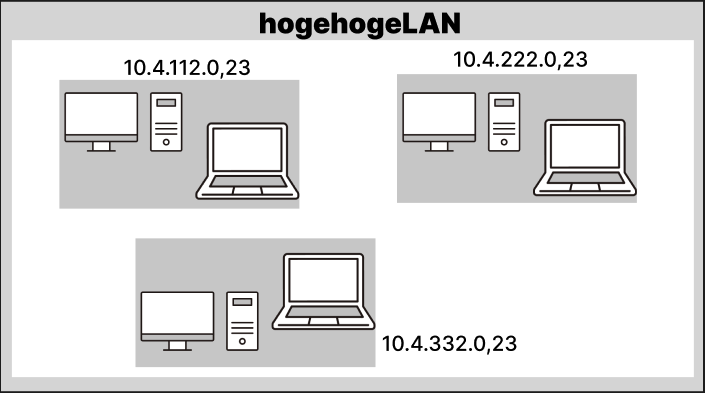
\includegraphics[width=10cm]{image/02-Body/network.png}
    \caption{同一LAN内でIPアドレスの違うネットワーク}
    \label{network}
\end{figure}

\subsection{事前準備}
事前に構造体とグローバル変数を定義しておきます。
\begin{tcolorbox}[breakable]
    \begin{verbatim}
1 type netowork struct {
2       RoomId int
3	    Ip     string
4	    Mask   int
5   }
6 type Option struct {
7	Address string
8 }
9
10 var count int
    \end{verbatim}
\end{tcolorbox}

\subsection{csvファイルからネットワーク一覧を取得}
今回は対象となるネットワークアドレスをcsvファイルに一覧として用意しておきます。
\begin{tcolorbox}[breakable]
    \begin{verbatim}
room_id, network, mask
1,10.4.112.0,23
2,10.4.222.0,23
    \end{verbatim}
\end{tcolorbox}
\begin{tcolorbox}[breakable]
    \begin{verbatim}
1 func getIpAndMask() []netowork {
2   file, err := os.Open("./network.csv")
3   if err != nil {
4	       log.Fatal(err)
5	    }
6	    defer file.Close()
7	    r := csv.NewReader(file)
8	    rows, err := r.ReadAll() // csvを一度に全て読み込む
9	    if err != nil {
10		    log.Fatal(err)
11	    }
12	    var net []netowork
13	    for i, v := range rows {
14		    if i == 0 {
15		    	continue
16		    }
17		    id, _ := strconv.Atoi(v[0])
18		    mask, _ := strconv.Atoi(v[2])
19		    n := netowork{
20			        RoomId: id,
21			        Ip:     v[1],
22			        Mask:   mask,
23		    }
24		    net = append(net, n)
25	    }
26	    return net
27   }
    \end{verbatim}
\end{tcolorbox}

\subsection{それぞれのネットワークのIPを取得}
ARPの時と同じ処理なので省略します。

\subsection{ネットワークのすべてのIPに対してエコーTypeでICMPプロトコルを実行}
エコーTypeの番号は8番で、pingコマンドで使われているものと同じです。
\begin{tcolorbox}[breakable]
    \begin{verbatim}
1 func Ping(ip string, m int) int {
2	    count = 0
3	    addr := &net.IPNet{
4		    IP:   net.ParseIP(ip).To4(),
5   		Mask: net.CIDRMask(m, 32),
6   	}
7
8	    out := ips(addr)
9
10	    c, err := icmp.ListenPacket("ip4:icmp", "0.0.0.0")
11	    if err != nil {
12		    panic(err)
13	    }
14  	defer c.Close()
15
16  	for _, v := range out {
17
18		    opt := Option{
19			    Address: v.String(),
20		    }
21		    ip, err := net.ResolveIPAddr("ip4", opt.Address)
22		    if err != nil {
23		    	panic(err)
24  		}
25
26		    go try(c, ip.IP)
27	    }
28 }
29
30 func try(c *icmp.PacketConn, ip net.IP) {
31	now := time.Now().UnixMilli()
32	result := make([]byte, binary.MaxVarintLen64)
33	binary.PutVarint(result, now)
34
35	msg := icmp.Message{
36		Type: ipv4.ICMPTypeEcho,
37		Code: 0,
38		Body: &icmp.Echo{
39			ID:   os.Getpid() & 0xffff,
40			Seq:  1,
41			Data: result,
42		},
43	}
44
45	msgBytes, err := msg.Marshal(nil)
46	if err != nil {
47		return
48	}
49	if _, err := c.WriteTo(
50        msgBytes, 
51        &net.IPAddr{IP: ip}
52        ); err != nil {
53		return
54	}
55 }
    \end{verbatim}
\end{tcolorbox}

\subsection{エコー応答の数を計測}
\begin{tcolorbox}[breakable]
    \begin{verbatim}
func Ping(ip string, m int) int {
            ・・・
    time.Sleep(time.Second)
        
    fmt.Println("現在の接続端末数:", count)
    return count  
}
        
func try(c *icmp.PacketConn, ip net.IP) {
        c.SetDeadline(time.Now().Add(time.Second))
        
        rb := make([]byte, 1500)
        n, _, _ := c.ReadFrom(rb)
        if err == nil {
                rm, err := icmp.ParseMessage(
                    ipv4.ICMPTypeEcho.Protocol(), 
                    rb[:n]
                    )
                if err == nil && 
                rm.Type == ipv4.ICMPTypeEchoReply {
                    echo, ok := rm.Body.(*icmp.Echo)
                    if ok {
                        t, _ := binary.Varint(echo.Data)
                        fmt.Println(
                            ip, ":",
                            time.Now().UnixMicro()-t*1000,
                            " ms"
                            )
                        if time.Now().UnixMilli()-t < 1000 {
                            count++
                        }
                    }
                }
        }
}
    \end{verbatim}
\end{tcolorbox}

\subsection{}

\chapter{おわりに}
\section{あとがき}

\section{参考文献}
\begin{thebibliography}{30}
\bibitem{icmp} \url{https://www.cloudflare.com/ja-jp/learning/ddos/glossary/internet-control-message-protocol-icmp}
\bibitem{rfc} \url{https://www.rfc-editor.org/rfc/rfc792.html}
\bibitem{arp_format} \url{https://www.n-study.com/tcp-ip/arp-format}
\bibitem{yokuwakaru} 福永勇二(2018)『ネットワークがよくわかる教科書』SBクリエイティブ株式会社発行
\bibitem{arpscan} \url{https://github.com/google/gopacket/blob/master/examples/arpscan/arpscan.go}
\bibitem{pgDora56} \url{https://github.com/pgDora56/PinGo}
\end{thebibliography}